\documentclass[12pt,reqno]{article}

\usepackage[usenames]{color}
\usepackage{amssymb}
\usepackage{amsmath}
\usepackage{amsthm}
\usepackage{amsfonts}
\usepackage{amscd}
\usepackage{graphicx}
\usepackage{mathrsfs}

\usepackage[colorlinks=true,
linkcolor=webgreen,
filecolor=webbrown,
citecolor=webgreen]{hyperref}

\definecolor{webgreen}{rgb}{0,.5,0}
\definecolor{webbrown}{rgb}{.6,0,0}

\usepackage{color}
\usepackage{fullpage}
\usepackage{float}

\usepackage{graphics}
\usepackage{latexsym}
\usepackage{epsf}
\usepackage{breakurl}

\setlength{\textwidth}{6.5in}
\setlength{\oddsidemargin}{.1in}
\setlength{\evensidemargin}{.1in}
\setlength{\topmargin}{-.1in}
\setlength{\textheight}{8.4in}

\newcommand{\seqnum}[1]{\href{https://oeis.org/#1}{\rm \underline{#1}}}

\newcommand{\N}{\mathbb{N}}
\newcommand{\Z}{\mathbb{Z}}
\newcommand{\R}{\mathbb{R}}
\newcommand{\xenc}{\mathrm{xenc}}
\let\up=\textsuperscript
\newcommand{\ct}{c}
\usepackage{bigints}
\def\restmod#1#2{#1\ (\mathrm{mod}\ #2)} %%% for the congruences


\begin{document}

\begin{center}
\epsfxsize=4in
\end{center}

\theoremstyle{plain}
\newtheorem{theorem}{Theorem}
\newtheorem{corollary}[theorem]{Corollary}
\newtheorem{lemma}[theorem]{Lemma}
\newtheorem{proposition}[theorem]{Proposition}

\theoremstyle{definition}
\newtheorem{definition}[theorem]{Definition}
\newtheorem{example}[theorem]{Example}
\newtheorem{conjecture}[theorem]{Conjecture}

\theoremstyle{remark}
\newtheorem{remark}[theorem]{Remark}

\begin{center}
\vskip 1cm{\Large\bf Some Patterns for Generating Permutations on the Natural Numbers
}
\vskip 1cm
\large
Robert Daland \\
Siri Natural Language Understanding \\
Apple, Inc \\
\href{mailto:r.daland@gmail.com}{\tt r.daland@gmail.com} 
\end{center}

\vskip .2 in

\begin{abstract}
Permutations on the natural numbers (hereafter: natperms) are theoretically uncountable. Despite this theoretical fecundity, concrete examples of natperms are not well exemplified in the literature. This paper begins by outlining some generator patterns for ``simple'' natperms. It is shown that for the base examples, the maximum distance between an element and its image is either constant or scales with the element's magnitude. Then the paper introduces a ``nonsimple'' natperm, in which the maximum displacement appears to scale supra-exponentially.

\end{abstract}

\section{Introduction}

What can a permutation on the natural numbers (a \textit{natperm}) look like? And what constraints does the structure of the natural numbers impose on the space of permutations of this countably infinite set? 

\section{Notation and conventions}

When it is necessary to distinguish the starting value for the natural numbers, the following notations will be used: \begin{itemize} 
  \item $\mathbb{N} = \{ 1, 2, \ldots \}$
  \item $\mathbb{N}_0 = \{ 0, 1, \ldots \}$
\end{itemize}
Both sets will be referred to as ``the natural numbers''. This article will take the domain for natperms to be $\mathbb{N}$, i.e. starting from $1$ rather than $0$.

The symbol $\pi$ will be used to denote generic natperms. Lowercase Greek letters will be used to denote specific natperms, with two notable exceptions: the add-1 map is denoted with $\sigma(n) = n + 1$, and the add-k map with $\sigma_k(n) = n + k$. These are exceptions because $\sigma$ and $\sigma_k$ are not natperms themselves (although this article will construct a variety of simple natperms from slight modifications of them).

The term \textbf{orbit} will refer to the collection of values generated by repeated application of a map, starting from some reference value. Orbits may include preimages of the reference value, i.e. a sequence of values may extend ``backwards'' when that is well-defined. The term \textbf{cycle} will be reserved for orbits in which the same value repeats after finitely many iterations of the map, i.e. $\pi^k(n) = n$ for some positive $k$. The \textbf{support} of a natperm is the set of values which are not fixed points. 

% The \textbf{displacement} of a permutation $\pi$ at a point $k$ is the distance between the point and its image, $|\pi(k) - k|$, or equivalently, the distance between two successive elements of an orbit. The \textbf{maximum displacement} is a function $\Delta_{\pi}(n) = \max_{1 \leq k \leq n} |\pi(k) - k|$.

Some of the examples discussed in this article can be represented as a product of \textit{disjoint} permutations. However, composition of permutations with overlapping support is generally out of scope.

\section{Patterns for generating natperms}

This section introduces various means of constructing ``simple'' natperms, usually with some kind of variation of $\sigma$.

\subsection{Finite natperms}

Let $\xi_0$ be a bijection on a subset of the natural numbers. Define the \textit{lifting} operation by constructing a natperm $\xi$ whose value is the same as $\xi_0$ on its domain, and the identity mapping elsewhere:
\begin{equation}
  \xi(n) = \begin{cases}
    \xi_0(n), & n \in domain(\xi_0) \\
    n, & \text{otherwise}
  \end{cases}
\end{equation}

A finite permutation is normally understood as a bijection on a set like $\{ 1, 2, \ldots, m \}$ for some $m$, i.e. what makes it finite is that the domain is finite. Every such bijection can be lifted to a natperm. In fact, it will prove convenient to apply the \textit{lifting convention} throughout this article: lifting will be understood to apply automatically to eligible mappings (those denoted by lowercase Greek letters, with the exception of $\sigma$/$\sigma_k$). As a result of this convention, the domain of a bijection on a subset of the natural numbers is effectively the entire natural numbers, which is not a finite set. In this context, the notion of finiteness must be scoped to the support of the natperm rather than its domain. Accordingly, $\xi$ is a \textit{finite natperm} if and only if $\exists M \in \mathbb{N} \ni | support(\xi) | \leq M$.

\subsection{Block cyclic natperms}

Let $(b_j)_{j=1}^{\infty}$ be an increasing sequence of natural numbers. The reader may visualize this sequence as partitioning the natural numbers into a sequence of contiguous blocks: the starting block $B_1 = \{ 1 \leq n < b_1 \}$, and successor blocks $B_j = \{ b_j \leq n < b_{j+1} \}$ for all $j > 1$. A natperm is obtained by defining some kind of permutation on each block. A simple approach is to use the add-1 mapping on each block, ``gluing'' the top of each block to its bottom. Formally, given the sequence values $(b_j)$, this is achieved as follows:

\begin{equation}
  \beta(n) = \begin{cases}
    b_j, & n = b_{j+1} - 1 \\
    n + 1, & \text{otherwise}
  \end{cases}
\end{equation}
This article will refer to such mappings as \textbf{block cyclic} natperms. 

The simplest example is the parity-swapping map, which can be compactly represented with the cycle notation as $\phi = (1 \ 2)(3 \ 4)(5 \ 6)\cdots$. Note that in the parity-swapping map, there is an upper bound on block size, i.e. it is a \textbf{bounded block cyclic} natperm.

It is also possible to define an \textbf{unbounded block cyclic} natperm. One way to do this is by setting the blocks to grow exponentially, e.g. $b_j = 2^j$.

\subsection{Shift-and-glue natperms}

Shift-and-glue natperms are closely related to the modulus group $\mathbb{Z}_k$, with some critical differences introduced by the fact that subsets of the natural numbers have a least element.

Let ${\lfloor n \rfloor}_k$ denote the orbit of the natural number $n$ under the add-k map $\sigma_k$, i.e. the set $\{ n, n + k, n + 2k, \ldots \}$. This article will refer to every such set as a \textbf{strand}. Note that ${\lfloor n \rfloor}_k \supset {\lfloor n + k \rfloor}_k$. More generally, if $n_1$ and $n_2$ are two distinct natural numbers, either ${\lfloor n_1 \rfloor}_k$ and ${\lfloor n_2 \rfloor}_k$ are disjoint, or they are in a subset-superset relationship. A \textbf{maximal strand} is a strand which is not contained in any other strand. With the convention that natural numbers start at 1, the maximal strands for $\sigma_k$ are ${\lfloor 1 \rfloor}_k$, ${\lfloor 2 \rfloor}_k$, $\ldots$, ${\lfloor k \rfloor}_k$. 

A shift-and-glue natperm is formed by gluing pairs of disjoint strands together. Gluing is accomplished by traversing one strand in descending order, switching over at the least elements, and traversing the other strand in ascending order. Here, ``traversing'' means that the natperm maps elements within a strand to the next larger or smaller element within the same strand. A simple example is given below:

\begin{equation}
    \nu(n) = \begin{cases}
        n - 2, & \text{if}\ n \text{ is even and greater than 2} \\
        1, & \text{if}\ n = 2 \\
        n + 2, & \text{if}\ n \text{ is odd} 
    \end{cases}
\end{equation}
The natperm can be more concisely represented by adopting a notational convention: if a strand appears on the left-hand side of a $\rightarrow$, it is traversed in decreasing order, while if it occurs on the right-hand side, it is traversed in ascending order. Thus, the natperm above can be written $\nu = {\lfloor 2 \rfloor}_2 \rightarrow {\lfloor 1 \rfloor}_2$.

Note that this convention excludes formulae like ${\lfloor 1 \rfloor}_3 \rightarrow {\lfloor 2 \rfloor}_3 \rightarrow {\lfloor 3 \rfloor}_3$, because that would imply that the same strand ${\lfloor 2 \rfloor}_3$ is traversed in both ascending and descending orders. However, because of the lifting convention, the formula ${\lfloor 1 \rfloor}_3 \rightarrow 2 \rightarrow {\lfloor 3 \rfloor}_3$ is allowed. This notation indicates that all elements of ${\lfloor 2 \rfloor}_3$ are subject to the identity mapping, except for $2$ itself.

This notation highlights that shift-and-glue natperms with $\sigma_k$-strands are closely related to permutations on the mod group $\mathbb{Z}_{k}$. The key difference is that strands have a traversal order (ascending, descending, or identity), and all non-identity strands must be paired off in ascending/descending pairs. A slightly more complex example is shown in Fig. \ref{fig:shiftandglue}, representing $\gamma = ( \lfloor 1 \rfloor_6 \rightarrow \lfloor 5 \rfloor_6 ) ( \lfloor 2 \rfloor_6 \rightarrow \lfloor 3 \rfloor_6 ) ( \lfloor 6 \rfloor_6 \rightarrow \lfloor 4 \rfloor_6 )$.

\begin{figure}
  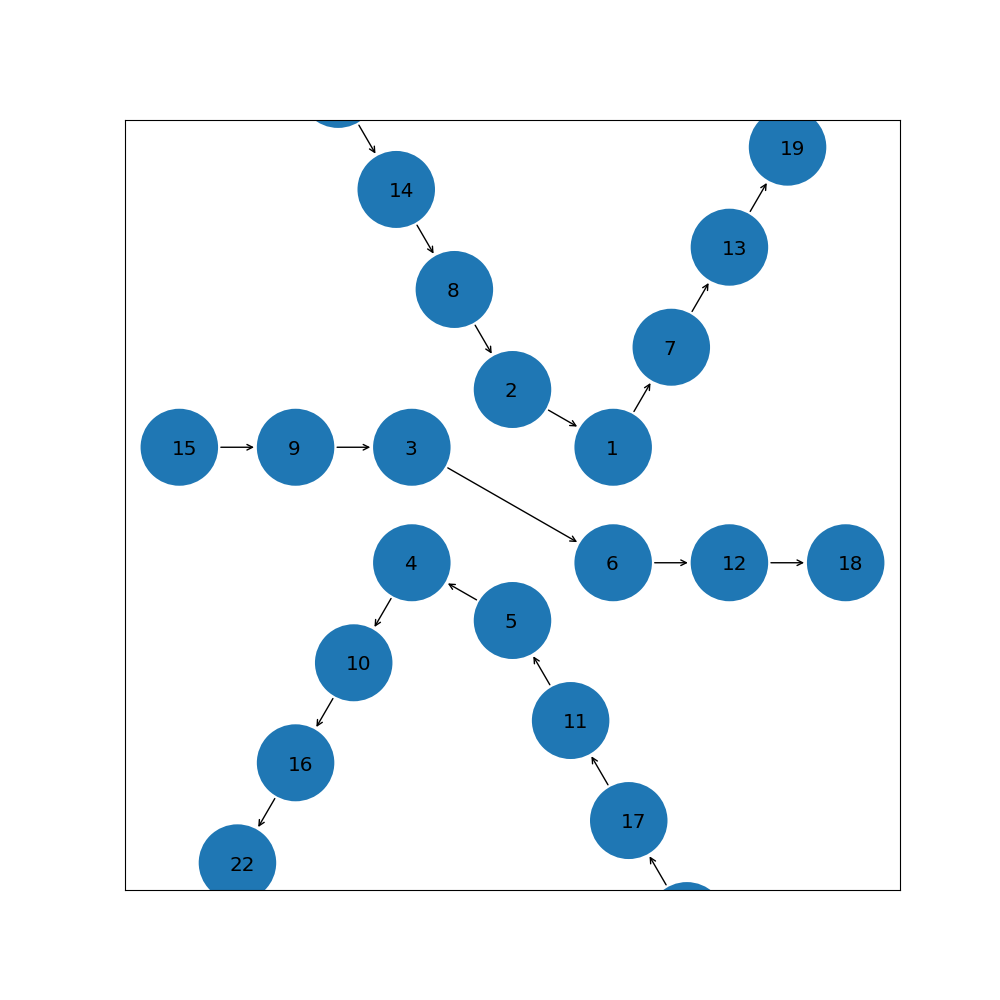
\includegraphics[width=\linewidth]{figs/fig1.png}
  \label{fig:shiftandglue}
  \caption{A shift-and-glue permutation.}
  \label{fig:shiftandglue}
\end{figure}

\section{Maximum displacement}

All of the examples presented in the previous section have the property that values are mapped to other, closeby values. The purpose of this section is to formalize what is meant by ``closeby''.

\subsection{Definition}

Let $\pi$ be a natperm. Define the \textit{displacement} of $\pi$ at an input $n$ as the distance between $n$ and $\pi(n)$. Then the maximum displacement (up to a given value $m$) is $\Delta_m(\pi) = \max_{n \leq m} | \pi(n) - n |$. This article will summarize the limit behavior using big-O notation, as follows.

\begin{center} \begin{tabular}{ |c|c|c| } 
  \hline
    verbal description & big-O notation       & definition \\
  \hline
    constant                & $\pi \in \Theta(1)$ & $\exists C \ni \lim_{m \rightarrow \infty} \Delta_m(\pi) = C$ \\
    scales linearly       & $\pi \in \Theta(n)$ & $\exists C \ni \lim_{m \rightarrow \infty} \frac{\Delta_m(\pi)}{m} = C$ \\
  \hline
\end{tabular} \end{center}

\subsection{Finite natperms}

\underline{Claim}: If $\pi$ is a finite natperm, then $\pi \in \Theta(1)$.

\textit{Proof}: By definition, the support of a finite natperm is a finite set $N$. If $N$ is empty (because $\pi$ is the identity mapping), the displacement is $0$ everywhere, and $\pi \in \Theta(1)$. Otherwise, $N$ must be nonempty. Since it is a finite, nonempty set of natural numbers, the max and min must be well-defined. The value $(\max(N) - \min(N))$ is an upper bound for the maximum displacement of $\pi$ on $N$. Thus, $\pi$ must achieve a maximum value $C \leq \max(N) - \min(N)$ for some value $m \in [ \min(N), \max(N) ] $, and the displacement is zero for all other values. Thus, the maximum displacement is $C$ and $\pi \in \Theta(1)$.

\subsection{Block cyclic natperms}

\underline{Claim}: If $\pi$ is a bounded block cyclic natperm, then $\pi \in \Theta(1)$.

\textit{Proof}: Let $(b_j)_{j=1}^{\infty}$ be the sequence of boundaries that define $\pi$. By the definition of bounded block cyclic natperm, there is an finite upper bound $C \ni | b_{j+1} - b_j | \leq C \forall j$. Since the natperm only remaps elements within a block, the maximum displacement can never exceed the maximum block size (which must be less than or equal to $C$).

\underline{Conjecture}: If $\pi$ is an unbounded block cyclic natperm, then $\pi \in \Theta(n)$ (or $\pi \in \Theta(1)$).

\textit{Rationale}: Consider the example provided earlier, where the blocks are defined by boundary sequence $b_j = 2^j$ and the mapping on each block is the shift map (except gluing the top of the block to its bottom). The first two blocks are $(1)$ and $(2)$. For all higher blocks $j > 2$, the displacement is $1$ within the block (the shift amount), and then $2^j - 2^{j-1} = 2^{j-1}$ at the glue point. Since $2^{j-1}$ is increasing in $j$ (and greater than $1$ for all $j > 1$), the maximum displacement is $2^{j-1}$ for values up to $2^j$. Therefore, at the glue points, the ratio of displacement to value is $2^{j-1} / 2^j = \frac{1}{2}$ (and elsewhere it tends to zero as $j$ increases). This shows that one-half is the limit value for the ratio of maximum displacement to value.

This unbounded block cyclic natperm was constructed to have the greatest possible displacement within blocks (by gluing top to bottom). And therefore the blockwise displacement scales linearly with the size of the blocks, even though the blocks themselves grow exponentially in size. And since the block sizes accumulate exponentially, the resulting ratio of maximum displacement to input size is linear too. This article will not attempt to prove that this property holds for all possible choices of block sizes. Instead, this is left as a conjecture for future research.

Finally note that by varying the blockwise permutation, it is possible to construct a block cyclic natperm with unbounded blocks, but finite maximum displacement. Let $[b_j, b_{j+1})$ be an arbitrary block. Partition the elements of this block by their parity (evens and odds), and define a blockwise permutation which traverses the evens in ascending order and the odds in descending order, gluing to the closest element at the top and bottom as necessary. For example, the block interval $[2, 8)$ would have the blockwise cycle $(2, 4, 6, 7, 5, 3)$ and the block interval $[1, 9)$ would instead have the cycle $(1, 2, 4, 6, 8, 7, 5, 3)$. The displacement is $2$ when traversing the interior of the block, and $1$ at glue/switch points. Therefore, it is always possible to make a blockwise natperm have finite/constant maximum displacement. The force of the conjecture is in the upper bound: regardless of the block boundaries and the blockwise permutations, the maximum displacement cannot be supra-linear in the input.

\subsection{Shift-and-glue natperms}

\underline{Claim}: If $\pi$ is a shift-and-glue natperm, $\pi \in \Theta(1)$.

\textit{Proof}: Let $\sigma_k$ be the shift map that generates the strands of $\pi$. For identity strands, the displacement is $0$, and for both ascending and descending strands, it is the constant value $k$. Recall that the glue points are in the interval $[1, k]$. The maximum possible displacement between glue points is therefore $|k - 1|$. Then $k$ is an upper bound for the displacement for all input values.

Note that this proof is designed for the base example presented earlier. It is also possible to generate shift-and-glue permutation which have more complex behavior in the ``center'', and eventually settle into similar behavior as the basic example. The details of the proof would need to be adjusted to handle such cases, although the general structure would remain the same. 

\subsection{Summary}

This section has presented a formalization of the notion of "locality" with respect to natperms. The basic idea is to track the distance between an element and its image. The maximum distance is of course finite in finite natperms. Block cyclic natperms can be considered as an infinite product of finite permutations. If the block size is upper bounded, the maximum distance is too; if not, it is conjectured that the maximum distance scales linearly with the input (or less; but crucially, not supra-linearly). Shift-and-glue natperms can be considered as a finite product of permutations on countably nonfinite subsets of $\mathbb{N}$; here, too, the maximum distance is finite. These ``simple'' examples are constructed from familiar elements (finite blocks, finite permutations, the shift map, and some light gluing operations). This raises an interesting question: is it possible to construct a natperm which is essentially different from these simple examples? For example, can there be a natperm $\pi$ which is not in $\Theta(n)$ or $\Theta(1)$? Can a natperm be a product of a mix of orbits which belong to different displacement classes?

\section{A natperm with nonlocal displacement}

The previous sections introduced various patterns for generating natperms, all exhibiting the property that the maximum displacement was either $O(1)$ or $O(n)$. The remainder of this paper describes a method to construct a natperm which seemingly lacks this locality property.

\subsection{Overview}

The general approach will start with a set $\mathbb{B}$ that is homeomorphic to $\mathbb{N}$. This article will refer to an invertible mapping from $\mathbb{N}$ onto $\mathbb{B}$ as an \textbf{encoder}, and its inverse as the corresponding \textbf{decoder}. Let \texttt{fenc}, \texttt{fdec} be an encoder-decoder pair, and \texttt{genc}, \texttt{gdec} another, different encoder-decoder pair. Then $\texttt{gdec} \circ \texttt{fenc}$ is a bijection from $\mathbb{N}$ to $\mathbb{N}$, in other words a natperm. The remainder of this section will define the bijective space $\mathbb{B}$, an encoder-decoder pair, a different encoder-decoder pair; finally it will conclude with some analysis.

\subsection{Canonical binary strings}

Define the set of \textbf{canonical binary strings} as follows:
\begin{equation}
  \mathbb{B} = \{ \langle 1s \rangle \, | \, s \in \{0,1\}^{*} \}
\end{equation}
where $*$ is the Kleene star operator (meaning any number of repetitions of any elements, including 0 repetitions). For clarity, strings will be delimited by angle brackets; thus $\langle \rangle$ denotes the empty string (which is not a canonical binary string), while $\langle 1 \rangle$ denotes the string consisting only of the symbol $1$.

\subsection{Binary encoder/decoder}

It is well known that a natural number can be represented as a sum of all powers of 2 up to some $k$, each multiplied by a coefficient that is either 0 or 1. For example:
\begin{equation}
  13 = (1 \cdot 2^3) + (1 \cdot 2^2) + (0 \cdot 2^1) + (1 \cdot 2^0)
\end{equation}
Define the binary encoder \texttt{benc} as mapping each natural number to the shortest such coefficient sequence (i.e. with no extraneous leading zeros), e.g. $\texttt{benc}(13) = \langle 1101 \rangle$.

The binary decoder \texttt{bdec} is simply the inverse of \texttt{benc}. Note that standard computational implementations of \texttt{benc} allow extraneous leading zeros. Items like $\langle 01101 \rangle$ and $\langle 001101 \rangle$ would otherwise map to the same value as $\langle 1101 \rangle$ does (13). But allowing this would prevent invertibility. The exclusion of leading zeros in $\mathbb{B}$, and the restriction of \texttt{benc} to the shortest binary coefficient sequence, is all so that \texttt{benc} and \texttt{bdec} can be inverses.

\subsection{Primefac Peano encoder/decoder}

This encoder will be defined by composing a number of simpler, invertible mappings (none of which are encoders themselves). Because each mapping in the encoder is invertible, it is straightforward the verify the encoder is 1-1. Finally it is demonstrated that the composed mapping is onto.

\subsubsection{Prime factorization}

It is well-known that every positive natural number can be factored into a product of primes. The factorization can be expressed in various ways, for example as a multiset:
\begin{equation}
28 = 7^1 \cdot 2^2 \rightarrow \begin{Bmatrix}
        2: & 2, \\
        7: & 1
    \end{Bmatrix}
\end {equation}
Since the primes are enumerable and totally ordered by $<$, it is also possible to represent the prime factorization with a \textbf{multiplicity vector}. In a multiplicity vector, the prime values are implicitly represented by the vector index; the corresponding value indicates the multiplicity. For example, $28 = (7^1) \cdot (5^0) \cdot (3^0) \cdot (2^2)$, so the multiplicity vector is $(1, 0, 0, 2)$. In this article, multiplicity vectors will be written with the final element corresponding to the lowest prime (2); values which appear to the left correspond to increasingly larger primes. In this way, leading zeros on the multiplicity vector correspond to leading zeros in a binary string: they do not change the value, and should be suppressed. Thus, a well-defined (and invertible) mapping is obtained by defining $primefac : \mathbb{N} \rightarrow \mathbb{N}_0^{*}$ as mapping integers to the shortest multiplicity vector that includes all nonzero multiplicities (in other words, with no leading zeros).

\subsubsection{Matchstick mapping}

A primitive method for representing positive integers is with a sequence of strokes; each stroke looks like the numeral $1$, and the number of strokes indicates the magnitude of the number. For example, $3 \rightarrow \langle 111 \rangle$. This paper will define the matchstick mapping $stick : \mathbb{N}_0 \rightarrow \mathbb{B}$ as mapping an integer $n$ to a string consisting of $n$ copies of the symbol $1$. Note that $stick(0) = \langle \rangle$. The Peano axioms define the natural numbers in a way that is closely related to the matchstick mapping.

Some papers follow the convention that a scalar function applies element-wise, if its argument is a vector. This paper will instead explicitly indicate that the function is meant to apply element-wise, by defining $\overline{stick} : \mathbb{N}_0^{*} \rightarrow \mathbb{B}^{*}$ explicitly: $\overline{stick}((n_1, n_2, \ldots, n_k)) = (stick(n_1), stick(n_2), \ldots, stick(n_k))$.

\subsubsection{String joining}

It is common to compose a sequence of strings into a single string. For example, simple concatenation is often represented with the $+$ operator, e.g. $\langle 1 \rangle + \langle 0 \rangle = \langle 10 \rangle$. Simple concatenation is not generally invertible. An alternative is to inserting a delimiter character at each join point. This paper will denote such a joining operation with the notation $\bigoplus_d$ symbol, where $d$ indicates the delimiter character. In this paper, the delimiter will be $0$. 
For example, $\bigoplus_0 (\langle 1 \rangle, \langle \rangle, \langle \rangle, \langle 11 \rangle) = \langle 100011 \rangle$. 

\subsubsection{Putting it all together}

The almost-correct definition of $\texttt{penc}(n) = \bigoplus_0 \, (\overline{stick} \circ primefac)(n)$. This mapping is illustrated with the ongoing example of $n = 28$.
\begin{center} \begin{tabular}{ |c| l cl cc cl c r| } 
  \hline
    input                &                &    &    &     &   28     &     &    &      &  \\
    primefac          &       (        & 1 & ,  & 0 & ,           & 0  & ,  &  2  & ) \\
  \hline
    stick                &                 & 1 &    &    &             &     &    & 11  & \\ 
    delimiters        &                 &    & 0 &    &    0       &     & 0 &      & \\
  \hline
    concatenation & $\langle$ &    &     &   & 100011 &    &     &      & $\rangle$ \\
  \hline
\end{tabular} \end{center}

There is an unfortunate problem with $1$, however. The unit $1$ has no prime factors, so its multiplicity vector is empty, so the concatenation is empty, and therefore does not belong to $\mathbb{B}$. This can be worked around by adding $1$ to the number before applying $primefac$. In other words, the final definition must be $\texttt{penc} = \bigoplus_0 \, (\overline{stick} \circ primefac \circ \sigma_1)$.

\subsubsection{Invertibility}

It is straightforward to show that \texttt{penc} is 1-1: \begin{itemize}
  \item $\sigma_1$ is 1-1
  \item $primefac$ is 1-1
  \item $\overline{stick}$ is 1-1
  \item $\bigoplus_0$ is 1-1 (since $stick$ outputs only the empty string and strings of $1$s)
\end{itemize}


To demonstrate invertibility, it is sufficient to show that \texttt{penc} is onto, i.e. an arbitrary element $b \in \mathbb{B}$ must have a preimage. Observe that $b = \langle 1 s_{k} s_{k-1} \cdots s_0 \rangle$, where each $s_i$ is either the delimiter $0$ or the matchstick $1$. If $b$ contains no zeros, it must be a string consisting of $k$ copies of $1$, where $k \geq 1$. In this case, $stick^{-1}(b) = k$, and $2^k \geq 2$. Then $\sigma^{-1}(2^k) = 2^k - 1 \geq 1\in \mathbb{N}$. Otherwise, the split-by-$0$ operation (which is the inverse of the join-with-$0$ operation) must produce a sequence of strings of the form $\langle 1* \rangle$. This follows because $b$ can consist only of $1$s and $0$s, and each $0$ is a delimiter. The matchstick mapping is invertible, e.g. $match^{-1}(\langle \rangle) = 0$ and $match^{-1}$ applied to a sequence of $k$ $1$s is simply $k$. Then $\overline{match}^{-1}$ produces a sequence of integers, of which the leftmost must be nonzero, and all values must be nonnegative integers. In other words, $\overline{match}^{-1}$ yields a multiplicity vector. The leftmost entry corresponds to a prime $p > 2$, and its multiplicity must be greater than or equal to 1. Therefore, the product (the inverse of $primefac$) is well-defined and greater than 1. As a result, $sigma^{-1}$ can be applied, yielding a value that is greater than or equal to 1. In other words, every value $b \in \mathbb{B}$ has a preimage under \texttt{penc}. Since \texttt{penc} is 1-1, this preimage is unique; in other words, $\texttt{pdec} = \texttt{penc}^{-1}$ is well-defined and \texttt{penc} is an encoder.

\subsubsection{Selected examples}

This subsection illustrates the encoding/decoding for a few values of interest. The Pythonic notation $(x, )$ is used to indicate a vector consisting of the single element $x$ (as distinct from a scalar $x$ which happens to be enclosed in parentheses for grouping clarity).

\begin{center} \begin{tabular}{l c l}
  $\texttt{penc}(0)$ &    & $(undefined)$ \\
  \\
  $\texttt{penc}(1)$ & = & $\bigoplus_0 \, (\overline{stick} \circ primefac \circ \sigma) (1) = \bigoplus_0 \, (\overline{stick} \circ primefac) (2) $ \\
                              & = & $\bigoplus_0 \, (\overline{stick} (\, (1,) \, )) = \bigoplus_0  \,( \, stick(1), \,) = \bigoplus_0 \, ( \, \langle 1 \rangle, )$ \\
                              & = & $\langle 1 \rangle$
\end{tabular} \end{center}

\end{document}

